% Chapter 4

\chapter{研究设计}
相比于传统的线性回归算法,机器学习方法更适合于本文的实证研究。在对于公司内在价值的预测过程中,线性回归模型将变量间的关系进行框定,会造成很大的偏误(Bias),一般而言,现实问题中的变量关系并不完全符合线性,或多或少都会呈现非线性趋势。再加上本文数据维度较高,数据量较大,并且伴有缺失值,
机器学习方法均能做到完美解决。

本文的统计方法基于经济学中的一价定律(Law of One Price),类似于任一资产定价模型,我们用合成股票(Synthetic Stock)或复制投资(Replicating Portfolio)的市场价值去代表股票的内在价值,因为每个投资组合的基本特征都与被评估公司的特征相同。
例如最简单的FCFF法便是进行证券市场上无风险(Risk-free)债券与产生无风险现金流资产之间的比较;在CAPM中,股票的复制投资组合是市场投资组合(Market Portfolio)与相同$\beta$值无风险资产的组合等\cite{rossSimpleApproachValuation1978}。

同样,在现有的基本面分析研究中,因子的选择较少,对于超额收益的攫取策略较为局限。近35年来已有多项研究证明了例如动量因子(Momentum)、市值因子(Size)等已有异象因子的有效性,针对这些因子的原因剖析也已经有了结果,例如投资者的过度自信(Overconfidence)与处置效应(Disposition Effect)从行为角度解释了动量因子\cite{danielInvestorPsychologySecurity1998, grinblattProspectTheoryMental2005}。
为了突破传统因子研究的局限性,本文创新采用财务指标去构建错误定价因子$M$,并以此进行资产定价与配置。该因子的构建不参杂任何的主观因素,均通过客观标准去进行优化选择。


\section{模型总体设计}
图~\ref{model}~展现了本文的总体设计流程,首先选取股票数据组成证券池,然后挑选公司相应的财务指标,运用BRTs模型进行内在价值的预测,以预测出的内在价值与市场价值的差额去构建错误定价因子$M$,后以该错误定价因子分组进行投资组合的配置,并以真实股票交易数据进行仿真。

\begin{figure}[htbp]
  \centering
    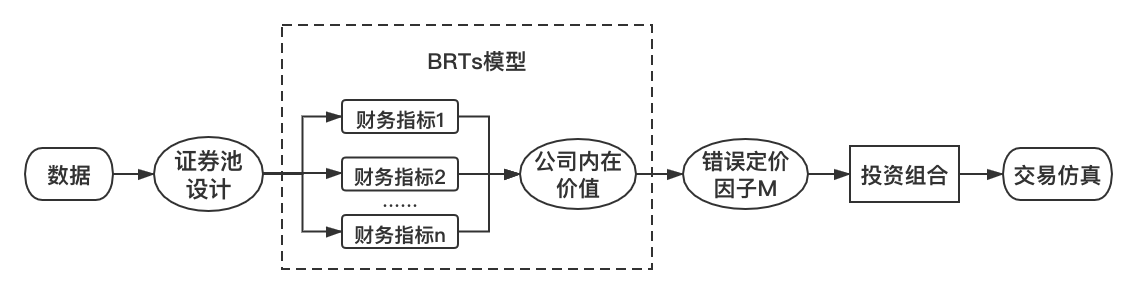
\includegraphics[width=\columnwidth]{毕业论文.png}
    \caption{模型总体设计}
    \label{model}
\end{figure}

\section{数据样本}
本文使用的A股公司财务报表数据和股票交易数据来自国泰安(CSMAR)数据库,因子模型数据分别来自中央财经大学金融学院\footnote{详见官网:\url{http://sf.cufe.edu.cn/info/1198/9562.htm}}、BetaPlus小组\footnote{详见官网:\url{https://www.factorwar.com/data/factor-models/}}以及WHUFT异象因子数据集\footnote{详见Github主页:\url{https://github.com/WHUFT}}。由于我国A股上市公司的季报数据自2002年起才开始公布,为了保障数据的完整性,本文财务指标数据以2002年第一季度为数据的起点,由于2020年12月财务数据较少,原因或在于公司财报未公布、数据库尚未更新完毕等,故最终选择以2019年12月为止。综上,本文数据样本时间区间为2002年3月至2019年12月,频次为季度。

对于股票样本的选择,本文以我国A股市场2018年底前上市的公司作为数据样本,规避未来收益数据的缺失。由于ST股票存在退市风险、金融行业公司财务报表结构有别于上市公司等原因,本文剔除掉ST股票、金融类股票,最后剩余3300支。

有关数据缺失部分,若某支股票在第$t$期市场价值$mktcap$数据存在缺失,则剔除该股票在$t$期的所有数据;但若有其他公司特征数据缺失,则由后文中所运用的机器学习算法BRTs进行自动填充。

在完成以上筛选步骤后,2002年3月至2019年12月的有效样本共132468条。图~\ref{size}~展示了2002年3月至2019年12月季频月度有效样本量。总体来看,每个月的样本量随年份呈现上升趋势,从2002年3月的938条有效样本增至2019年12月的3225条。

\begin{figure}[htbp]
  \centering
    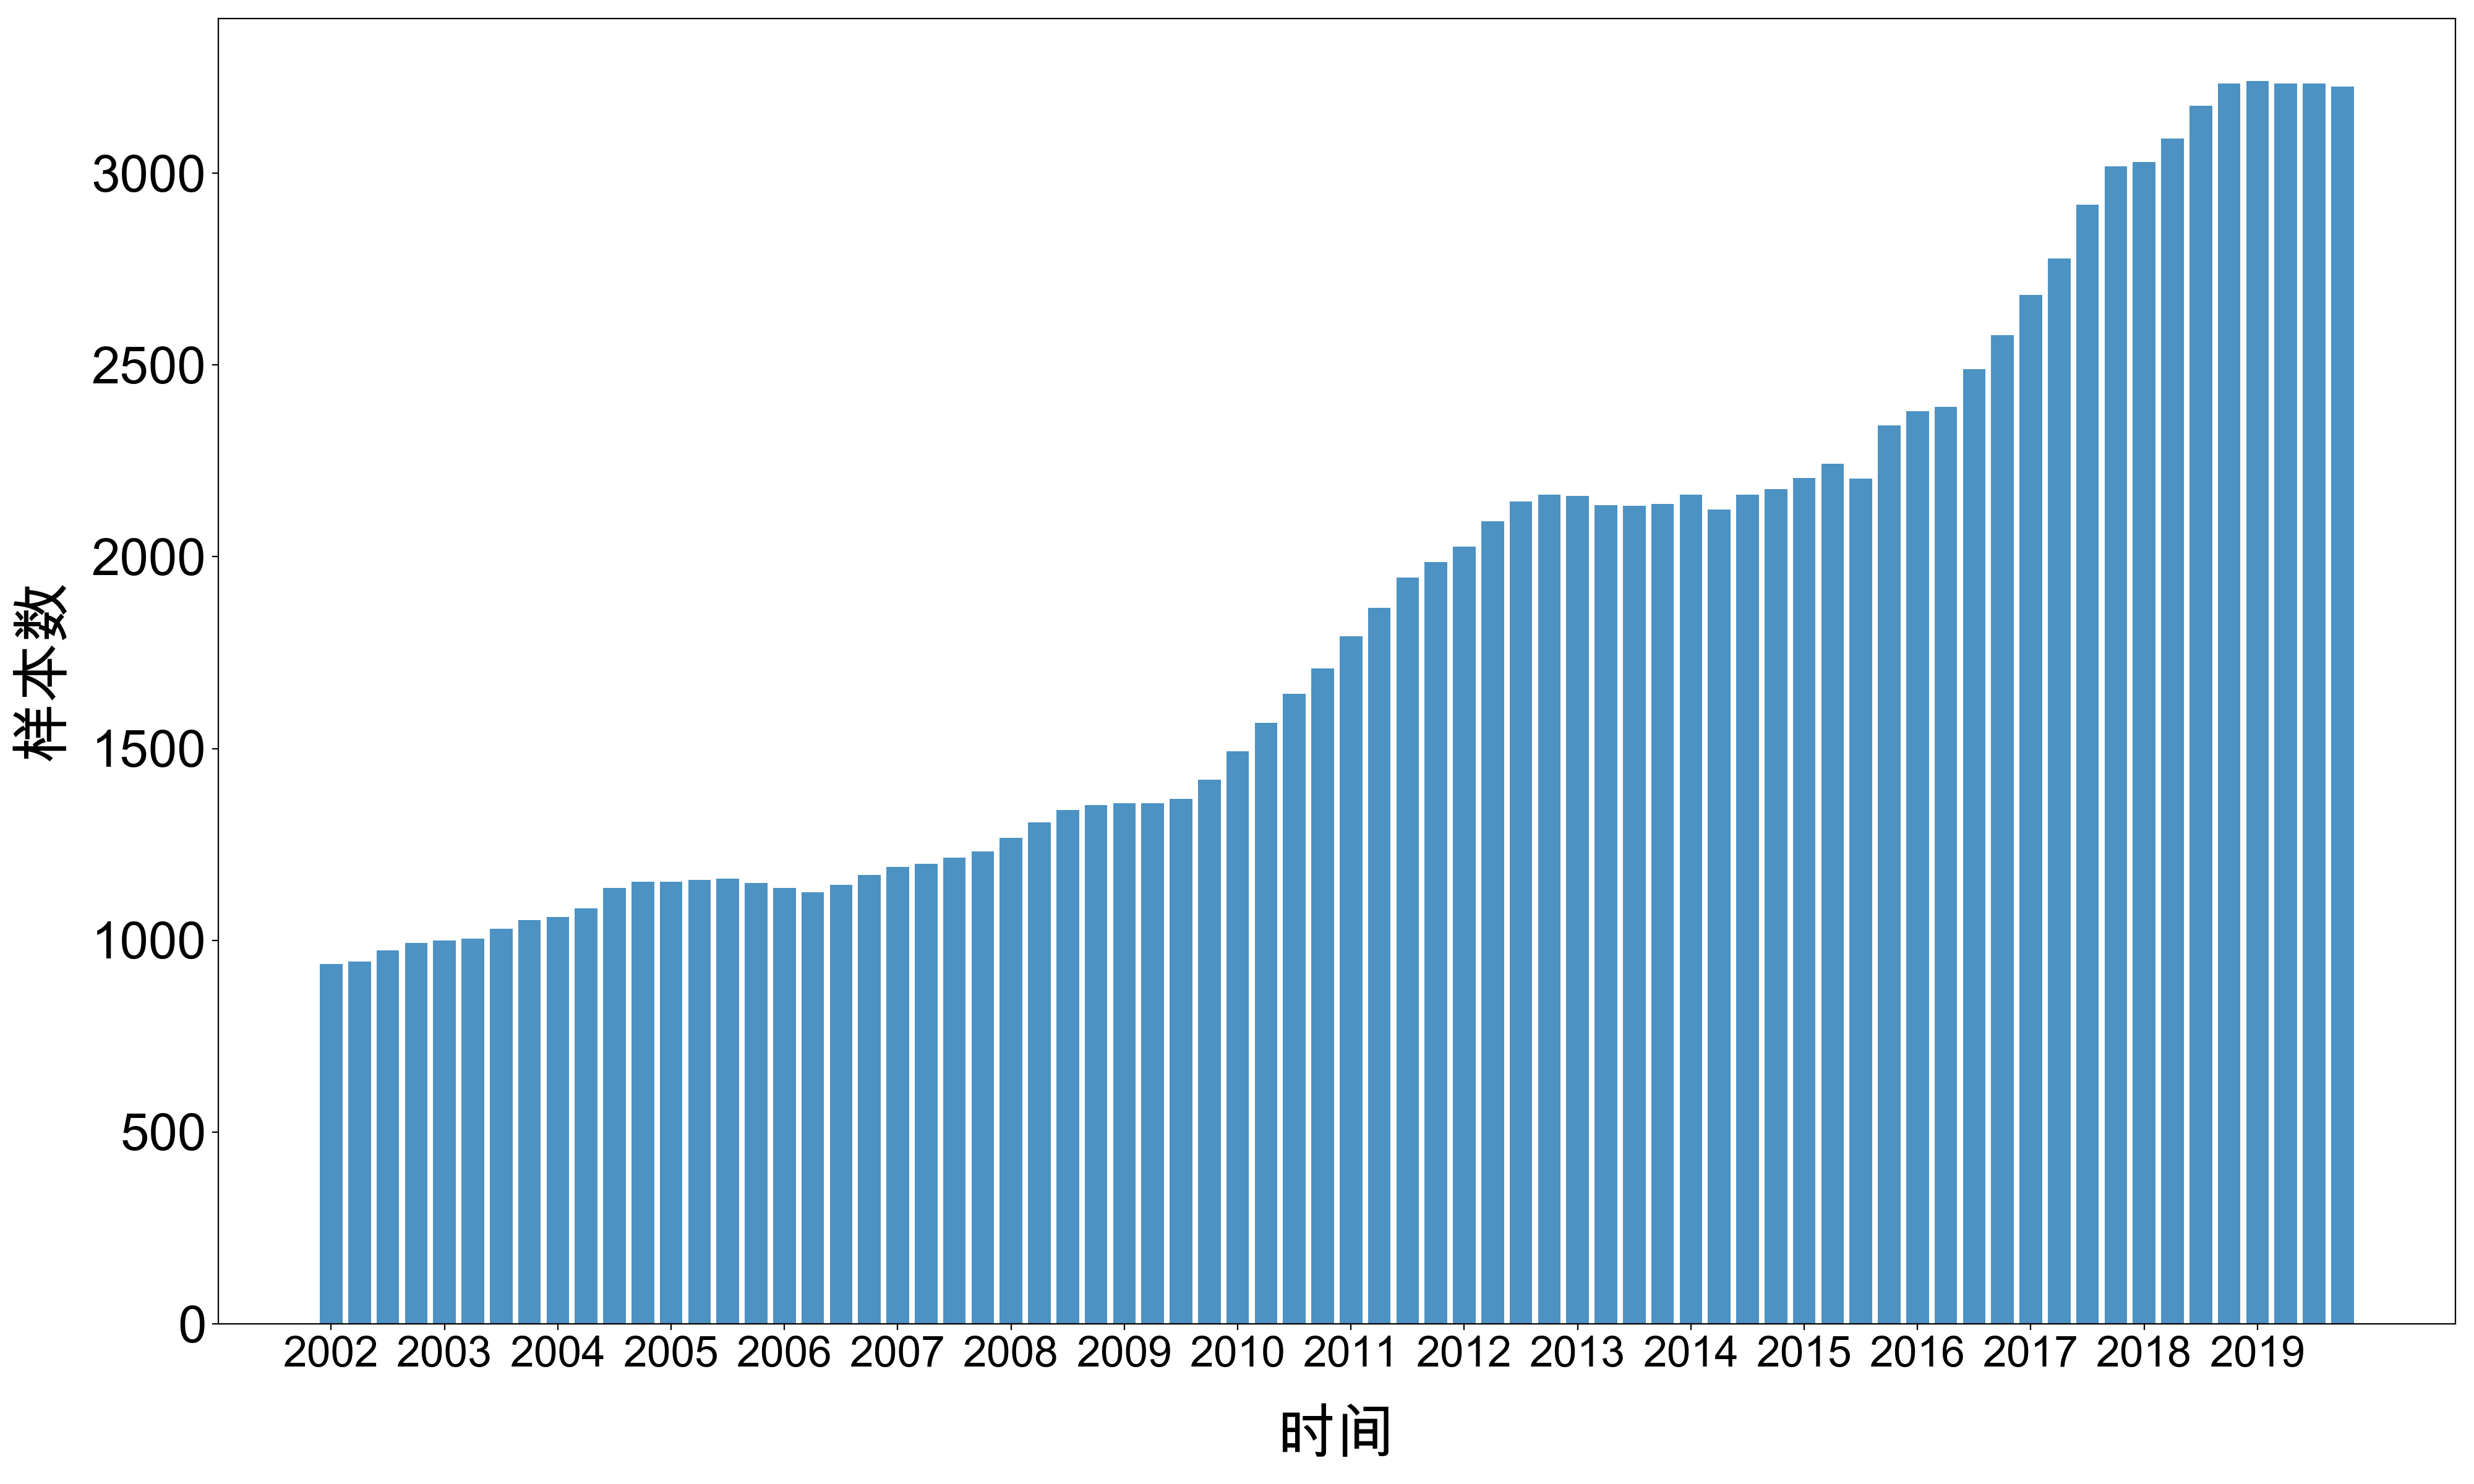
\includegraphics[width=\columnwidth]{sample_size.png}
    \caption{样本数据的月度有效样本量}
    \label{size}
\end{figure}

\section{变量定义与说明}
为了计算公司的错误定价因子$M$,首先需要对公司的内在价值进行估计。本文以公司市场价值为因变量,财务指标为自变量进行回归计算,得到的残差即为错误定价;之后通过Fama-MacBeth截面回归、因子模型回归等方法验证错误定价因子M的有效性。文章中采用的主要变量如表~\ref{variable}~所示。
\begin{table}[htbp]
  \centering
  \caption{变量定义与说明}
  \label{variable}
  \begin{tabular*}{0.9\hsize}{@{\hskip\tabcolsep\extracolsep\fill}*{2}{c}}
    \toprule
    变量名 & 定义及说明   \\
    \midrule
   $ mktcap_{it} $  & 公司$i$于第$t$期的市场价值  \\
   $M_{i, t}$  & 公司$i$于第$t$期的错误定价因子  \\
    $R_{i, t}$  &公司$i$于第$t$期月个股收益率  \\
    $BM$ & 市净率\\
    $beta $  & 市场投资组合$\beta$值 \\
    $grltnoa$ & 净经营性资产增长率\\
    $PA  $   & 毛利率\\
    $EP$   & 市盈率 \\
    $lagretn$ &上一个月的收益率\\
    $mom12$ &t-12月至t-2月的累计收益率(共计11个月) \\
    $mom36$ & t-36月至t-13月累计收益率(共计24个月)\\
          \bottomrule
  \end{tabular*}
\end{table}

\section{模型设定}
现有研究中,常见的公司内在价值计算方法包括现金流贴现法、相对价值法、经济附加值法、实物期权法等。这些方法虽然能起到一定的预测作用,但由于其选择的指标过少、过于死板,或太过于依赖使用者对未来的主观预测结果,亦或计算方法过于程式化等原因,很难排除掉数据窥视带来的影响。

根据本文的基本面分析原理,公司内在价值反映在一系列财务指标中,如式~\ref{eq1}~所示,其中$i$代表不同公司,$t$代表不同期数。$mktcap_{i, t}$ 为公司$i$于季度$t$时的市场价值,$f(.)$定义了一个参数为$\theta$的非线性函数,在本文中为采用BRTs方法背后具体的函数形式,参数$\theta$主要包括树的数量$n\_estimators$、学习率$learning\_rate$以及树的深度$max\_depth$,均采用网格调参的方法进行最优化,$ I_{i, t}=( I_{i, t,1},I_{i, t,2},...,I_{i, t,N})$代表公司$i$在第$t$期时$N$个财务指标向量,$\epsilon_{i, t}$为残差项。
\begin{equation}
\label{eq1}
mktcap_{i, t} =f(I_{i, t};\theta)+\epsilon_{i, t} 
\end{equation}

对于财务指标的选择,为避免数据窥视的影响,并非由笔者主观挑选。相反,本文于CSMAR数据库下载了所有财务报表数据,包括资产负债表、利润表与直接法和间接法计算的现金流量表,共计279个指标。但由于不同公司个体财务情况差异大、过于细分的指标数据未被使用、或是数据库数据录入缺失等原因,数据库中每个指标或多或少都有缺失值的存在,故为了计算的严谨性,将对279个财务指标进行统一筛选。

基于统计,在所有财务指标中,缺失值比例最大的达到99.99\%,最小为0.01\%,均值高达44.7\%,说明有很多指标数据缺失情况严重,具体情况详见附录~\ref{miss}。
为了做到对公司内在价值的准确评估,本文选择缺失值比例较小的指标,以避免缺失值造成的数据偏误\cite{yanFundamentalAnalysisCrossSection2017a};同时,为了能完整对公司内在价值进行评估,所选择的财务指标必须多样化。综上,本文以5\%的缺失值比例为界限,挑选出缺失值比例小于等于5\%的所有指标,共有51个,具体可见附录~\ref{missing}~。

在成功确定函数形式$f(.)$后,即完成对公司内在价值的预测后,将进行式~\ref{eq1}~的回归,以确定该期的错误定价情况。回归后残差即为公司市值与内在价值的偏差,将该残差基于市值进行标准化后的负值,定义为错误定价因子$M$,如式~\ref{eq2}~所示。
\begin{equation}
\label{eq2}
M_{i, t} =-1 \times \frac{\epsilon_{i, t}}{mktcap_{i, t}}
\end{equation}

当公司内在价值低于市场价值时,即残差大于0,对应$M$为负值,说明股票被高估;当公司内在价值高于市场价值时,$M$为正值,说明股票被低估。

其中,考虑到市场以及公司的变化情况,公司的内在价值以及错误定价因子$M$每期都会重新计算一次,并对公司进行重新分组调整,避免数据偏误。

总而言之,本文的统计方法不会偏好特定的股票市场、不考虑整个市场在特定期数是否被高估或低估、也不依赖于内在价值的理论模型。相反,本文将公司进行相互比较,使用拟合优度的统计标准来识别公司内在价值如何体现于会计属性。

后续研究中,每期都将根据错误定价因子$M$大小进行公司分组:Q1到Q5五组。其中Q1为$M$最小的公司,即股票最被高估;Q5为$M$最大的公司,即股票最被低估。如果基本面分析有效、财务指标蕴含公司的内在价值,当市场价值最终趋近于内在价值时,最被高估的股票价格会回落,最被低估的股票价格会爬升,以此构建低买高卖的投资组合来获利。

为验证上述猜想,后文将进行因子模型回归、Fama-MacBeth横截面回归以及稳健性分析,如式~\ref{eq3}、\ref{eq4}~所示。
\begin{equation}
\label{eq3}
R_{i, t+1}=a_{t}+b_{t} M_{i, t}+\sum_{k=1}^{K} c_{k, t} X_{i, k, t}+\epsilon_{i, t+1}
\end{equation}
\begin{equation}
\label{eq4}
R_{i, t}=\alpha_{i}+\sum_{k=1}^{K} \beta_{i, k} F_{k, t}+\epsilon_{i, t}
\end{equation}

式~\ref{eq3}~中$X_{i, k, t}$代表公司$i$于季度$t$时第$k$个公司特征,作为控制变量,具体特征见表~\ref{variable}~所示;若$b_{t}$显著,说明错误定价因子M能够有效预测股票价格未来走势,证明了其有效性。

式~\ref{eq4}~中$F_{k,t}$为季度$t$时第$k$个因子值,本文主要采用Fama-French 三因子模型、Carhart 四因子模型、Fama-French 五因子模型、以及Hou-Xue-Zhang 四因子模型(后称为q-因子模型)进行分析;其中$\alpha_{i}$代表该投资组合的超额收益。如果Q1到Q5五组超额收益$\alpha$有显著的递增趋势,以及Q1、Q5的多空组合超额收益$\alpha$显著大于0,也能证明错误定价因子$M$的有效性。

\section{描述性统计}
表~\ref{description}~列出了使用LightGBM算法对数据进行模拟后,所有相关变量的描述性统计值,这里将样本根据错误定价因子$M$分成了Q1到Q5五组进行考察。其中第一列为所有数据的平均值,第二列为相应变量与错误定价因子$M$的相关系数,第三列为Q1组(价值最被高估)的变量平均值,一直到最后一列为Q5组(价值最被低估)的变量平均值。

\setlength{\tabcolsep}{1.2mm}{
\begin{table}[htbp]\centering
\def\sym#1{\ifmmode^{#1}\else\(^{#1}\)\fi}
\caption{描述性统计}
\label{description}
\begin{tabular*}{\hsize}{@{\hskip\tabcolsep\extracolsep\fill}*{8}{c}}
\toprule
               &\multicolumn{1}{c}{}&\multicolumn{1}{c}{}&\multicolumn{5}{c}{错误定价因子$M$分组}\\\cline{4-8} 
          &\multicolumn{1}{c}{所有数据}&\multicolumn{1}{c}{相关系数}&\multicolumn{1}{c}{Q1 (被高估)}&\multicolumn{1}{c}{Q2}&\multicolumn{1}{c}{Q3}&\multicolumn{1}{c}{Q4}&\multicolumn{1}{c}{Q5 (被低估)}\\
          &\multicolumn{1}{c}{(1)}&\multicolumn{1}{c}{(2)}&\multicolumn{1}{c}{(3)}&\multicolumn{1}{c}{(4)}&\multicolumn{1}{c}{(5)}&\multicolumn{1}{c}{(6)}&\multicolumn{1}{c}{(7)}\\
\midrule
$M$       &   0.4296 &    1.000&  -0.3173&  -0.0157&   0.2372&   0.5847&   1.6615\\
$mktcap $  &  7.1297&   -0.112& 15.2640&   8.5644&   5.8529&   3.8186&   2.1325\\
$R_{t}$   &    0.8750 &   -0.032&   2.6395&   1.1614&   0.5074&   0.2173&  -0.1539\\
$R_{t+1}$ & 0.7814&    0.040&   0.2792&   0.4824&   0.7857&   0.9555&   1.4064\\
$R_{t+2}$ & 0.7266&    0.038&   0.4140&   0.4454&   0.5725&   1.0322&   1.1706\\
$lagretn $  &   0.0295&    0.012&   0.0387&   0.0268&   0.0252&   0.0239&  0.0328\\
$BM$    &    0.4304&    0.069&   0.3321&   0.4351&   0.4755&   0.4871&   0.4230\\
$EP  $      &  0.0190&   -0.051&   0.0190&   0.0223&   0.0207&   0.0179&   0.0148\\
$beta$     &  1.1420&   -0.006&   1.1063&   1.1414&   1.1485&   1.1555&   1.1609\\
$grltnoa$ &   1.4602&    0.020&   0.3031&   0.3421&   0.2945&   1.9855&   5.0868\\
$PA$        & 0.0133 &   -0.071&   0.0179&   0.0153&   0.0114&   0.0093&   0.0123\\
\bottomrule
\end{tabular*}
\end{table}
}

在描述性统计表中,从第三列到最后一列,第$t-1$期到第$t$期的收益$R_t$逐渐减少,说明购买被高估的股票收益更高,与现实情况相符,同时第$t$期前一个月的收益$lagretn$也基本呈现逐渐减少的趋势。但是第$t$期到第$t+1$期的收益$R_{t+1}$、$t+1$期到第$t+2$期的收益$R_{t+2}$逐渐增加,说明被高估的股票价格下降,逐渐趋于正常,所以收益变低,而被低估的股票价值上涨到正常价值,收益变高,与本文猜想保持一致。

%%%
相比于被高估的Q1组股票,被低估的Q5组股票平均有着更高的市净率$BM$、更低的市场价值$mktcap$;再加上错误定价因子$M$与市净率$BM$有着正相关关系,说明被高估的股票更多是高市值的价值股,而被低估的股票多是低市值的成长股。

错误定价因子$M$与$beta$相关系数为负,说明系统性风险并不能解释$M$对于股票未来收益的预测能力。由于$M$与其他异象的相关系数基本都低于0.05,在后续回归中,将$beta$值、过去一个月的收益$lagretn$、市净率$BM$、市盈率$EP$、净经营性资产增长率$grltnoa$以及毛利率$PA$作为公司层面的控制变量。由于公司市值$mktcap$与错误定价因子$M$高度相关,在后续回归中为避免多重共线性问题,控制变量将不包含公司市值$mktcap$。
%%%




%\subsection{原始代码}
%朴实的代码块:
%
%使用 verbatim 环境可以得到如下原样的输出。
%\begin{verbatim}
%print("Hello world!")
%\end{verbatim}
%
%使用 listings 包提供的 lstlisting 环境可以对代码进行进一步的格式化,minted 包所提供的 minted 环境还可以对代码进行高亮。更多定制功能请自行参照文档配置。
%
%\subsection{算法描述/伪代码}
%参考 \href{https://en.wikibooks.org/wiki/LaTeX/Algorithms}{Algorithms} 与 algorithm2e 文档,给出一个简单的示例,见算法 \ref{alg:alg1}。
%
%\begin{algorithm}
%  \SetAlgoLined
%  \KwData{this text}
%  \KwResult{how to write algorithm with \LaTeXe}
%  initialization\;
%  \While{not at end of this document}{
%    read current\;
%    \eIf{understand}{
%      go to next section\;
%      current section becomes this one\;
%    }{
%      go back to the beginning of current section\;
%    }
%  }
%  \caption{如何写算法}\label{alg:alg1}
%\end{algorithm}
%
%\section{绘图}
%关于使用 \LaTeX{} 绘图的更多例子,请参考 \href{https://www.overleaf.com/learn/latex/Pgfplots_package}{Pgfplots package}。一般建议使用如 Photoshop、PowerPoint 等制图,再转换成 PDF 等格式插入。
%
%\section{写在最后}
%工具不重要,对工具的合理运用才重要。希望本模板对大家的论文写作有所帮助。
